\documentclass[a4paper,fleqn]{cas-dc}
\usepackage{graphicx}
\usepackage{float}
%\documentclass[a4paper,fleqn,longmktitle]{cas-dc}
\usepackage[numbers]{natbib}
%\usepackage[authoryear]{natbib}
%\usepackage[authoryear,longnamesfirst]{natbib}

%%%Author macros
\def\tsc#1{\csdef{#1}{\textsc{\lowercase{#1}}\xspace}}
\tsc{WGM}
\tsc{QE}
%%%

\begin{document}
\let\WriteBookmarks\relax
\def\floatpagepagefraction{1}
\def\textpagefraction{.001}
\let\printorcid\relax % 可去掉页面下方的ORCID(s)

% Short title
% \shorttitle{<short title of the paper for running head>} 
\shorttitle{}    

% Short author
% \shortauthors{<short author list for running head>}
\shortauthors{Zhen Wang et al.}

%论文标题
\title[mode = title]{VersionGS: Archive and Replay for Evolving 3D Gaussian Map}  

%作者信息
\author[1]{Zhen Wang}
\author[1]{XXX}
\author[2]{XXX}
\author[2]{XXX}
\cormark[1]

\address[1]{Xi'an Polytechnic University, Xi'an  710000‌, China} %声明第一单位
\address[2]{xxx Laboratory, xxx University, Changsha 410073, China} %声明第二单位
\cortext[1]{Corresponding author}  %声明通讯作者


% Here goes the abstract
\begin{abstract}
In this work we demonstrate $a_b$ the formation Y\_1 of a new type of polariton on the interface between a cuprous oxide slab and a polystyrene micro-sphere placed on the slab. The evanescent field of the resonant whispering gallery mode of the micro sphere has a substantial gradient, and therefore effectively couples with the quadrupole $1^S$ excitons in cuprous oxide. This evanescent polariton has a long life-time, which is determined only by its excitonic and component. The polariton lower branch has a well pronounced minimum. This suggests that this excitation is localized and can be utilized for possible. The spatial coherence of the polariton can be improved by assembling the micro-spheres into a linear chain.
The polariton lower branch has a well pronounced minimum. This suggests that this excitation is localized and can be utilized for possible. The spatial coherence of the polariton can be improved by assembling the micro-spheres into a linear chain.
\end{abstract}

% Use if graphical abstract is present
%\begin{graphicalabstract}
%\includegraphics{}
%\end{graphicalabstract}

% Research highlights
% \begin{highlights}
% \item highlight-1
% \item highlight-2
% \item highlight-3
% \end{highlights}

% Keywords
% Each keyword is seperated by \sep
\begin{keywords}
keyword-1 \sep 
keyword-2 \sep 
keyword-3
\end{keywords}

\maketitle

\section{Introduction}

3D Gaussian Splatting (3DGS) provides a high-quality and efficient
representation for reconstructing and rendering three-dimensional
environments. Its ability to represent both scene geometry and
appearance makes it attractive for long-term applications such as
robotic mapping and augmented reality. In these applications, however,
the environment may change over time: objects can be added, removed,
or moved, and local appearance can vary between mapping sessions.
When a mapping system updates its representation using new
observations, overwriting the previous map may erase the last recorded
state of the environment. Preserving historical map versions would
support applications such as querying past scenes, restoring earlier
maps, comparing recorded states, and evaluating mapping algorithms
against previously constructed maps.

Existing methods address several aspects of evolving scenes, but
they provide different guarantees for historical access. Online
mappers such as GaME~\cite{yugay2026game} adapt the current map by
adding new geometry, removing outdated Gaussians, and suppressing
stale observations. Continual methods provide additional support for
scene history: CL-Splats~\cite{ackermann2025clsplats} recovers past
states by recording local changes, while
GaussianUpdate~\cite{zeng2025gaussianupdate} and
LTGS~\cite{kim2026ltgs} represent past scenes using Gaussian visibility
and shared object templates, respectively. These approaches support
map updates or historical rendering through specific update rules or
shared scene representations. Dynamic Gaussian
representations~\cite{luiten2024dynamic,wu2024gaussians} also enable
rendering at different timestamps through trajectories or
time-conditioned deformations. However, the ability to query a
timestamp does not by itself guarantee that a previously committed
map state remains unchanged after subsequent optimization.

A straightforward way to preserve immutable states is to store each
map version as an independent snapshot. This approach permits direct
access and exact recovery, but its storage cost grows with the
cumulative size of all versions. Delta-based storage can reduce
redundancy, yet cross-version parameter correspondence becomes
difficult when Gaussian topology changes. Moreover, recovering a
version from a chain of deltas may require applying intermediate
updates. Thus, it remains challenging to preserve immutable Gaussian
map versions, share storage across updates, and directly replay any
committed version.

Achieving these properties requires addressing two related challenges.
First, Gaussians do not have stable identities by default.
Densification creates Gaussians through cloning and splitting, while
pruning and scene updates remove existing ones. These operations
change the number and ordering of Gaussians, so a tensor row cannot
reliably identify the same Gaussian across versions. Second, parameter
changes do not necessarily correspond to changes in the scene.
Continued optimization may adjust the positions, shapes, and
appearance of Gaussians even in regions where the environment has
remained unchanged. Preserving every such parameter update limits
cross-version sharing, whereas reusing earlier parameters may affect
the quality of the newly committed map. A versioning system must
therefore track Gaussians across topology-changing updates and decide
which parameters can be reused while accounting for their effect on
map quality.

% \begin{center}
% 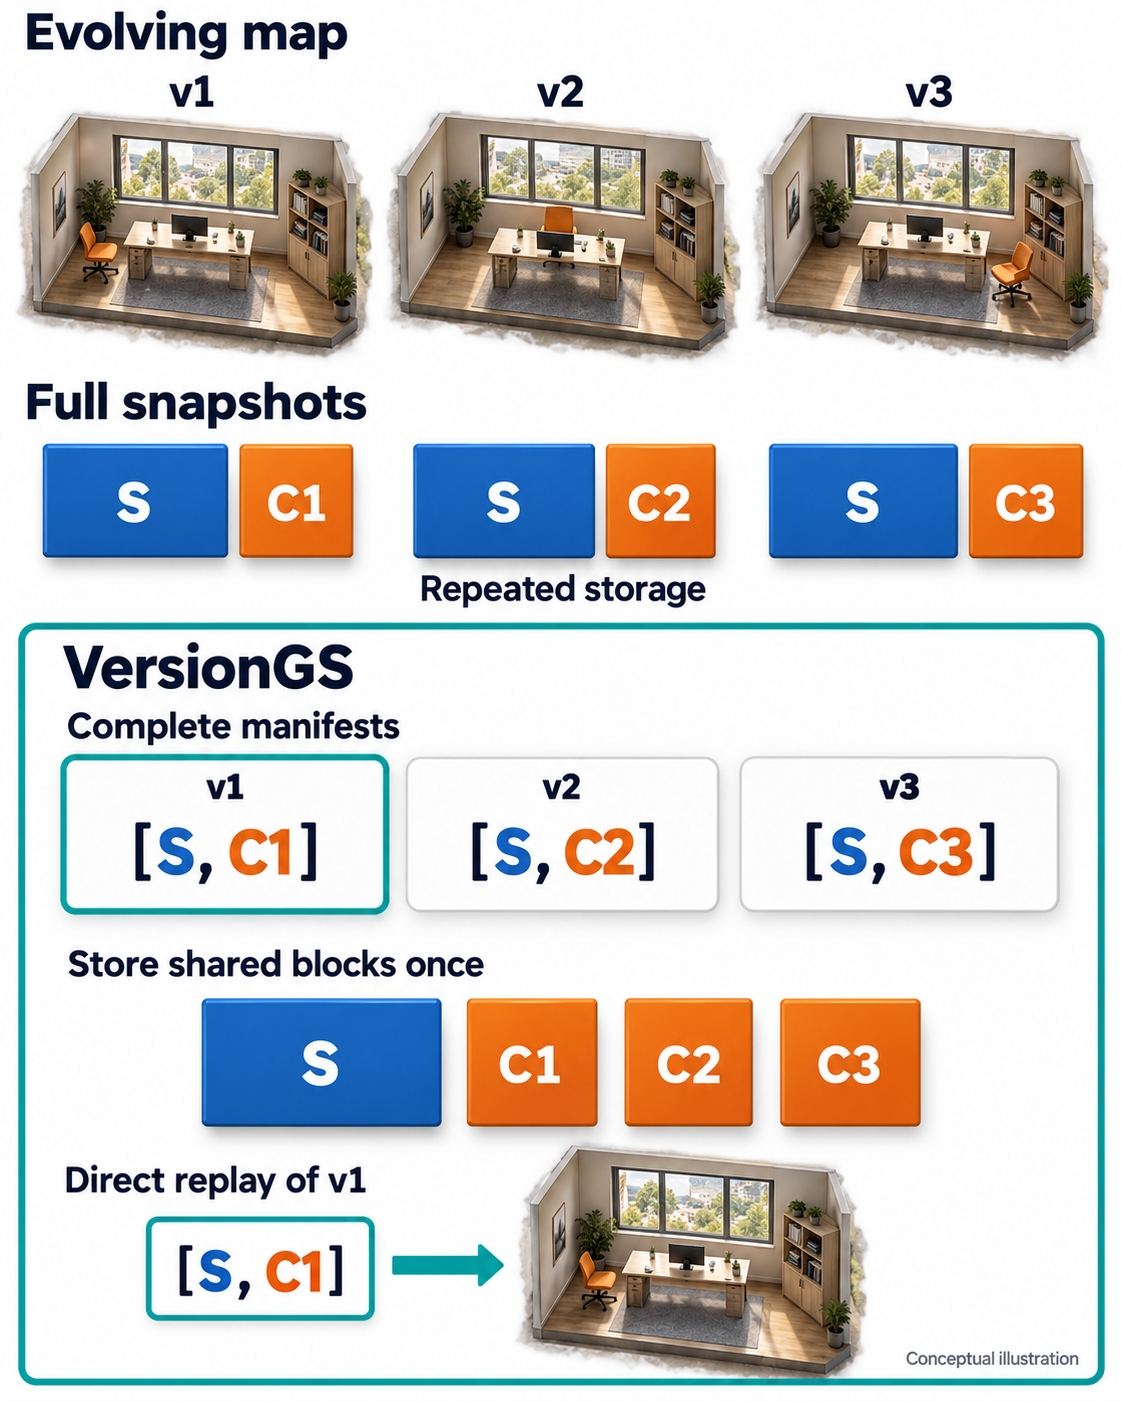
\includegraphics[width=\columnwidth]{section/01_TeaserFigure.png}
% \end{center}




To address these challenges, we present \textbf{VersionGS}, a
framework for archiving and replaying evolving 3D Gaussian maps.
Its central design is to make every committed version logically
complete while sharing identical content across versions in physical
storage. VersionGS separates the live map being optimized from its
committed versions, so subsequent updates do not alter earlier
commits. It assigns persistent identities to Gaussians, allowing
them to be tracked across updates even when their tensor rows change.
When constructing a new version, VersionGS uses scene-change evidence
and visibility to select parameters from the current map or reuse
parameters from the previous commit. New Gaussians and regions
identified as changed use current parameters; for other regions,
the framework reuses earlier parameters where possible and checks
rendering quality to limit the impact of reuse.

\begin{figure}[H]
\centering
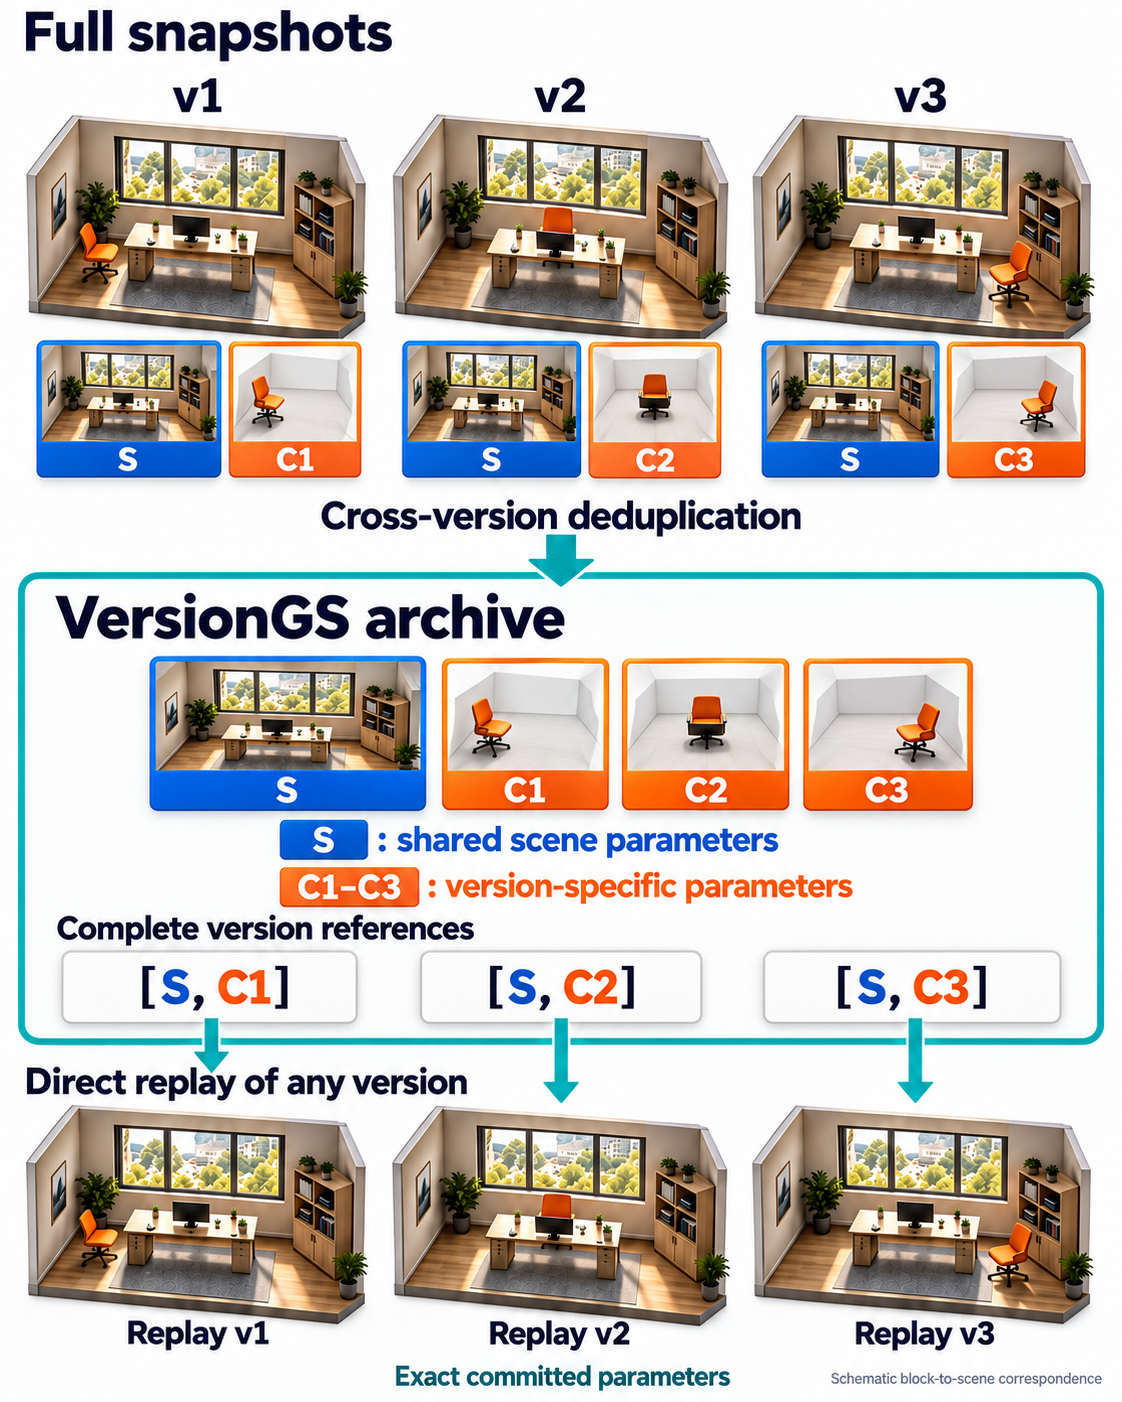
\includegraphics[width=\columnwidth]{figures/01_TeaserFigure_v3.png}
\caption{Example Image}
\label{fig:example}
\end{figure}

The resulting committed version may therefore differ from the live
map. Once committed, however, its selected parameters are stored
losslessly. Each version is represented by a complete manifest of
references to Gaussian parameter blocks, and identical blocks are
stored only once through content addressing. This design enables
exact recovery and direct rendering of any committed version without
the original observations or replaying intermediate updates.

We evaluate VersionGS on [datasets] across [number] successive map
versions. Our experiments measure the rendering quality of current
and historical versions, total archive storage, and the time required
to save and load a version. We compare against full snapshots,
compressed snapshots, and delta-based storage to evaluate the
benefits and costs of cross-version sharing. VersionGS reduces
archive storage by [X] compared with [baseline], while keeping
current-version rendering quality within [Y] dB of the underlying
mapper. We also verify that committed parameters are recovered
exactly and that historical versions remain unchanged after further
map updates.

Our contributions are threefold:
\begin{enumerate}
    \item We formulate the problem of archiving evolving 3D Gaussian
    maps as immutable, directly accessible versions despite
    topology-changing updates.

    \item We introduce persistent Gaussian identities and a
    change-aware version construction method that uses change
    evidence, visibility, and rendering-quality checks to guide
    parameter reuse across versions.

    \item We develop a lossless multi-version archive based on
    complete version manifests and content-addressed Gaussian
    parameter blocks, enabling exact replay of committed versions
    without the original observations or intermediate updates.
\end{enumerate}

\section{Related Work}



\section{Method}

\subsection{Problem Setup and Overview}
\label{sec:problem_setup}


3D Gaussian Splatting (3DGS) is an effective approach for 3D scene representation and novel view synthesis. In the method proposed by Kerbl et al., a static scene is reconstructed using a set of 3D Gaussians initialized from sparse points obtained through Structure-from-Motion (SfM) and subsequently optimized via differentiable rendering with multi-view supervision.
It represents the scene as a set of Gaussian primitives,
$\mathcal{G}=\{g_i\}_{i=1}^{N}$, where each Gaussian has parameters
\begin{equation}
    \boldsymbol{\theta}_i =
    (\boldsymbol{\mu}_i,\boldsymbol{s}_i,\boldsymbol{q}_i,
    \alpha_i,\boldsymbol{h}_i).
\end{equation}
Here, $\boldsymbol{\mu}_i$ is the position,
$\boldsymbol{s}_i$ and $\boldsymbol{q}_i$ describe its scale and rotation,
$\alpha_i$ is the opacity, and $\boldsymbol{h}_i$ contains spherical
harmonic coefficients for view-dependent color.
A differentiable renderer projects these Gaussians into an image,
and their parameters are optimized to match the input observations.
During training, densification and pruning also change the number
of Gaussians.

In an evolving environment, a single fixed reconstruction is no
longer sufficient.
New observations may reveal added, removed, or rearranged objects,
requiring both Gaussian parameters and the set of primitives to change.
We consider a stream of posed RGB-D observations,
\begin{equation}
    \mathcal{O} =
    \{(I_t,D_t,T_t,K_t)\}_{t=1}^{T},
\end{equation}
where $I_t$ and $D_t$ are the RGB and depth images,
$T_t$ is the camera pose, and $K_t$ contains the camera intrinsics.
An online mapper processes these observations to maintain a live map
that reflects the latest observed scene.
Our goal is to preserve a sequence of renderable map versions
while allowing this live map to continue updating.

We distinguish the live map $\mathcal{L}_k$ from the committed map
$\mathcal{C}_k$ at the $k$-th commit.
The live map remains available for further optimization,
whereas a committed map stays unchanged after it is saved.
The index $k$ denotes a chosen commit point, such as the end of a
capture session, rather than the time when a physical scene change
occurred.
A committed map need not be an identical copy of the live map:
it may reuse parameters from the previous commit when doing so
keeps rendering quality within a chosen tolerance.
This reduces storage caused by parameter changes in otherwise
unchanged parts of the scene.

VersionGS constructs each new commit from the current live map
and the previous committed map:
\begin{equation}
    \mathcal{C}_k =
    \operatorname{Build}
    (\mathcal{L}_k,\mathcal{C}_{k-1},\mathcal{E}_k,\mathcal{V}_k),
\end{equation}
where $\mathcal{E}_k$ contains detected scene-change evidence
since the previous commit, and $\mathcal{V}_k$ contains observations
used to check visibility and rendering quality.
The first commit is taken directly from the live map.
For later commits, persistent Gaussian IDs establish correspondence
across versions.
Change evidence, visibility, and quality checks then determine
which previous parameters can be reused.

Finally, VersionGS stores each commit as a complete list of references
to Gaussian parameter blocks.
Identical blocks are shared across versions and stored without loss.
Given a commit index $k$ and a camera specification $\pi$,
the archive restores $\mathcal{C}_k$ and renders
\begin{equation}
    (\hat{I},\hat{D},\hat{A})
    = \mathcal{R}(\mathcal{C}_k,\pi),
\end{equation}
where $\hat{I}$, $\hat{D}$, and $\hat{A}$ are the rendered color,
depth, and opacity.
Replay requires neither the original RGB-D observations nor
the application of intermediate updates.
The archive preserves the committed parameters exactly;
the quality tolerance applies only when constructing a commit
from the live map.

\subsection{Persistent Gaussian Identities}
\label{sec:gaussian_identities}

Standard 3DGS stores Gaussian parameters as rows in tensors.
These row indices are useful during optimization, but cannot reliably
identify Gaussians across map versions.
Adding or removing a Gaussian changes the tensor layout, while
densification creates new primitives through cloning and splitting.
As a result, the same row index may refer to different Gaussians
in different versions.
We therefore assign each Gaussian a persistent ID that is independent
of its tensor row and parameter values.

\paragraph{ID assignment.}
Each newly created Gaussian receives a unique integer ID, $u$.
IDs are assigned in increasing order and are never reused.
We represent a versioned Gaussian as
\begin{equation}
    g_u =
    (u,\boldsymbol{\theta}_u,p_u,\boldsymbol{r}_u,b_u),
\end{equation}
where $\boldsymbol{\theta}_u$ contains its rendering parameters,
$p_u$ is its parent ID, $\boldsymbol{r}_u$ is a region label,
and $b_u$ is its creation commit index.
The ID remains fixed as the Gaussian's position, shape, opacity,
and color are optimized.
All identity fields are stored alongside the parameter tensors
and undergo the same row insertions, removals, and reorderings.

\paragraph{Creation and removal.}
Gaussians initialized from newly observed geometry receive fresh IDs
and have no parent, denoted by $p_u=-1$.
Cloning and splitting also assign fresh IDs to the generated Gaussians,
with their parent IDs pointing to the source Gaussian.
Thus, a child records its origin without being treated as the same
primitive as its parent.
When a Gaussian is removed, we record its ID, retirement commit,
and removal reason.
These reasons distinguish scene removal from operations such as
densification and opacity-based pruning.
Removing a Gaussian from the live map does not alter any previously
saved commit.

\paragraph{Region labels.}
We use a coarse region label to associate Gaussians with detected
scene changes.
For a Gaussian created directly from an observation, the label is
assigned from its initial position:
\begin{equation}
    \boldsymbol{r}_u =
    \left\lfloor
    \frac{\boldsymbol{\mu}_u^{\mathrm{birth}}}{\ell}
    \right\rfloor,
\end{equation}
where $\ell$ is the grid cell size and the floor operation is applied
to each coordinate.
Gaussians produced by cloning or splitting inherit the source
Gaussian's region label.
This label remains fixed during later optimization.
It groups related primitives for change-aware version construction;
it is neither a semantic object label nor a continuously updated
spatial index.

\paragraph{Cross-version correspondence.}
Let $U_k^{\mathrm{live}}$ and $U_{k-1}^{\mathrm{commit}}$ denote the
Gaussian IDs in the current live map and the previous commit.
Their intersection identifies primitives present in both states:
\begin{equation}
    U_k^{\mathrm{shared}}
    =
    U_k^{\mathrm{live}}
    \cap U_{k-1}^{\mathrm{commit}}.
\end{equation}
IDs found only in the live map identify new primitives, while IDs
found only in the previous commit identify primitives no longer
present in the live map.
This correspondence allows us to retrieve previous parameters
even when tensor layouts differ.
A shared ID does not imply unchanged parameters or an unchanged
physical scene.
In the next section, we use scene-change evidence, visibility,
and rendering-quality checks to decide whether those previous
parameters can be reused.


\subsection{Change-Aware Version Construction}
\label{sec:version_construction}

Persistent IDs establish correspondence across versions, but a shared
ID does not tell us whether its previous parameters are still suitable.
A Gaussian may have changed because the scene changed, or simply
because optimization refined its parameters.
We therefore construct each new commit using both scene-change evidence
and rendering-quality checks.
The process starts from the current live map and selectively replaces
parameters with those from the previous commit.
It operates on a separate candidate map and leaves the live parameters
unchanged.

\paragraph{Change evidence and visibility.}
Let $U_k^{\mathrm{live}}$ and $U_{k-1}^{\mathrm{commit}}$ be the ID sets
of the current live map and the previous commit.
We collect the region labels associated with detected changes since
the previous commit into a set $\mathcal{Q}_k$.
For each current Gaussian $u$, we define a change flag
\begin{equation}
    c_u = \mathbb{1}[\boldsymbol{r}_u \in \mathcal{Q}_k].
\end{equation}
A positive flag means that the Gaussian belongs to a region supported
by change evidence.
The absence of this flag does not establish that the region is unchanged.

We also render the live map from selected observations in
$\mathcal{V}_k$.
A Gaussian is marked as visible if the renderer reports it as visible
in at least one of these views:
\begin{equation}
    v_u =
    \mathbb{1}\!\left[
        u \text{ is visible in any selected view}
    \right].
\end{equation}
This flag describes visibility in the selected observations,
rather than in all possible views.

\paragraph{Initial candidate.}
We initialize a candidate map $\widetilde{\mathcal{C}}_k$
from the live map $\mathcal{L}_k$.
New Gaussians and Gaussians in regions with detected changes retain
their current parameters.
For Gaussians present in both states, we initially reuse previous
parameters only when they are not visible and have no change flag:
\begin{equation}
    \widetilde{\boldsymbol{\theta}}_{u,k}
    =
    \begin{cases}
        \boldsymbol{\theta}_{u,k-1}^{\mathrm{commit}},
        & u \in U_{k-1}^{\mathrm{commit}},\
          c_u=0,\ v_u=0,\\[2pt]
        \boldsymbol{\theta}_{u,k}^{\mathrm{live}},
        & \text{otherwise}.
    \end{cases}
    \label{eq:initial_version}
\end{equation}
The candidate contains the same Gaussian IDs as the live map:
\begin{equation}
    U_k^{\mathrm{candidate}} = U_k^{\mathrm{live}}.
\end{equation}
Gaussians that exist only in the previous commit are therefore not
added back to the new version.
They remain available through their earlier commits.
Reusing parameters in currently invisible regions is an initial
choice; the complete candidate must still pass the quality check below.

\paragraph{Testing reuse in visible regions.}
Visible Gaussians without detected changes may also be able to reuse
previous parameters.
We collect these candidates as
\begin{equation}
    \mathcal{S}_k =
    \left\{
        u \in
        U_k^{\mathrm{live}} \cap U_{k-1}^{\mathrm{commit}}
        \;\middle|\;
        c_u=0,\ v_u=1
    \right\}.
\end{equation}
To avoid testing every Gaussian separately, we group eligible IDs
by the fixed UID intervals used by the archive.
Within each group, we measure the largest absolute parameter difference
between the live and previous states.
We test groups with smaller differences first and limit the number
of trials to control commit time.

For each trial, we replace the eligible Gaussians' parameters in
the current candidate with their previous values.
This produces a trial map $\mathcal{C}'_k$.
We accept the replacement only if its rendering quality stays within
the allowed degradation relative to the live map.
Otherwise, we undo the replacement.
Accepted replacements remain in the candidate during later trials,
so each check accounts for the combined effect of reuse.

\paragraph{Rendering-quality check.}
For each checking view $j$, we render both $\mathcal{L}_k$ and
$\mathcal{C}'_k$ and compare them with the observed RGB-D image.
We measure degradation using PSNR, SSIM, and depth mean absolute error:
\begin{align}
    d_j^{P}
    &=
    \operatorname{PSNR}_j(\mathcal{L}_k)
    -
    \operatorname{PSNR}_j(\mathcal{C}'_k),\\
    d_j^{S}
    &=
    \operatorname{SSIM}_j(\mathcal{L}_k)
    -
    \operatorname{SSIM}_j(\mathcal{C}'_k),\\
    d_j^{D}
    &=
    \operatorname{MAE}_j(\mathcal{C}'_k)
    -
    \operatorname{MAE}_j(\mathcal{L}_k).
\end{align}
Depth error is measured in meters over valid observed depth pixels.
For all three metrics, a positive difference indicates worse quality.

We use bootstrap resampling of the per-view differences to make
the decision less dependent on their mean alone.
Let $U_{.95}(d)$ denote the 95th percentile of the resampled means.
A trial passes when
\begin{equation}
    \begin{aligned}
        U_{.95}(d^{P}) &\leq \epsilon_P,\\
        U_{.95}(d^{S}) &\leq \epsilon_S,\\
        U_{.95}(d^{D}) &\leq \epsilon_D,
    \end{aligned}
    \label{eq:reuse_quality}
\end{equation}
where $\epsilon_P$, $\epsilon_S$, and $\epsilon_D$ are the allowed
quality drops.
Every trial is compared with the original live map, rather than
the previous trial.
This prevents successive replacements from each consuming a new
quality allowance.
The check provides empirical control on the selected observations;
it does not guarantee the same bound at unseen viewpoints.

\paragraph{Final commit.}
After the trials, we check the complete candidate using
Eq.~\eqref{eq:reuse_quality}.
If it passes, we use it as the new committed map.
Otherwise, we fall back to the live map:
\begin{equation}
    \mathcal{C}_k =
    \begin{cases}
        \widetilde{\mathcal{C}}_k,
        & \text{if the final candidate passes},\\
        \mathcal{L}_k,
        & \text{otherwise}.
    \end{cases}
\end{equation}
The first commit is taken directly from the live map because no
previous version is available.
Once constructed, $\mathcal{C}_k$ is stored without loss and remains
fixed during later mapping.
Reusing previous parameters creates opportunities for exact block
sharing, which we describe next.

\subsection{Shared Archive and Direct Replay}
\label{sec:archive_replay}

After constructing a committed map $\mathcal{C}_k$, we store it
in a shared archive.
Each commit describes a complete renderable map, while identical
parameter blocks are stored only once.
This separates the logical map version from its physical storage:
loading a version requires its block references, rather than
a sequence of changes from other versions.

\paragraph{Blocks based on persistent IDs.}
Splitting parameter tensors by row index can reduce sharing when
Gaussians are inserted, removed, or reordered.
We instead partition each committed map using fixed UID intervals.
For a block width $B$, interval $b$ contains
\begin{equation}
    \mathcal{B}_{k,b}
    =
    \left\{
        g_u \in \mathcal{C}_k
        \;\middle|\;
        bB \leq u < (b+1)B
    \right\}.
\end{equation}
Empty intervals are skipped, and Gaussians within each block
are sorted by UID.
Thus, moving a Gaussian to a different tensor row does not change
its block assignment or its order within that block.

Each block stores the Gaussian rendering parameters together with
their IDs, parent IDs, region labels, and creation commit indices.
Rendering parameters retain their original float32 values,
and identity fields are stored as int64 values.
Global settings, including the spherical harmonic degree,
are stored in the commit header.

\paragraph{Exact block sharing.}
We serialize each block in a fixed field order and compute
a content hash from its raw bytes and UID-range information:
\begin{equation}
    h_{k,b}
    =
    H\!\left(
        \operatorname{range}_{k,b}
        \,\Vert\,
        \operatorname{bytes}(\mathcal{B}_{k,b})
    \right),
\end{equation}
where $H$ is SHA-256 and $\Vert$ denotes concatenation.
If the archive already contains this hash, the new commit references
the existing block.
Otherwise, we compress the raw bytes using a lossless codec
and append the new block to the archive.
An index records each stored block's location and size.

Block sharing requires identical contents, including identity metadata.
Similar parameters or similar rendered images alone are not sufficient.
The version construction in Sec.~\ref{sec:version_construction}
encourages sharing by restoring selected previous parameters.
However, reusing some Gaussians within a block does not necessarily
make the whole block identical.
A block with any remaining content change is stored as a new block.

\paragraph{Complete commit manifests.}
For each version, we save a manifest containing its header,
commit metadata, and the complete ordered list of block references:
\begin{equation}
    M_k =
    \left(
        \operatorname{header}_k,\,
        \operatorname{metadata}_k,\,
        [h_{k,1},\ldots,h_{k,n_k}]
    \right).
\end{equation}
Here, $n_k$ is the number of nonempty blocks in the version.
The manifest also records the parent commit for bookkeeping,
but loading does not require loading that parent.
New commits add manifests and previously unseen blocks;
they do not modify the contents referenced by earlier commits.

The total storage consists of unique compressed blocks,
commit manifests, and the archive index:
\begin{equation}
    S_{\mathrm{archive}}
    =
    \sum_{h\in\mathcal{H}} S_{\mathrm{block}}(h)
    +
    \sum_k S_{\mathrm{manifest}}(M_k)
    +
    S_{\mathrm{index}},
\end{equation}
where $\mathcal{H}$ is the set of stored block hashes.
Unchanged blocks therefore contribute storage only once,
regardless of how many versions reference them.
The savings depend on how much block content remains identical
across commits.

\paragraph{Direct replay.}
To restore version $k$, we read its manifest, load and decompress
the referenced blocks, and concatenate their fields in UID order.
The header supplies the global settings needed to rebuild
the Gaussian model.
This recovers the committed parameters and identity metadata exactly,
without applying intermediate updates.
The archive contains the rendering state and version metadata,
but does not require optimizer states, training keyframes,
or the original RGB-D observations.

Given a camera specification $\pi$, including its pose, intrinsics,
and image size, the restored map can render color, depth, and opacity:
\begin{equation}
    (\hat{I},\hat{D},\hat{A})
    =
    \mathcal{R}\!\left(
        \operatorname{Load}(\mathcal{A},k),\pi
    \right).
\end{equation}
Loading requires reading the blocks of the selected version,
but does not require traversing its parent commits.
Its data-loading cost therefore depends on the selected map
and its compressed blocks, rather than the number of intervening
map updates.

The archive introduces no quantization or parameter approximation.
Any quality difference from the live map arises during version
construction, not during storage or recovery.
Exact parameter recovery is distinct from bit-exact rendered output,
which also depends on the renderer and execution environment.


\subsection{Mapping and Commit Procedure}
\label{sec:mapping_procedure}

\paragraph{Live map updates.}
We use GaME~\cite{yugay2026game} as the mapping backbone.
Given posed RGB-D observations and instance masks, it selects
keyframes, adds new geometry, removes outdated Gaussians,
and masks stale observations during optimization.
VersionGS maintains Gaussian identities throughout these operations
and records detected changes for version construction.
Before removing Gaussians, it records their IDs and region labels.
Newly created Gaussians receive fresh IDs.
Camera poses are supplied with the observations.

\paragraph{Keeping reusable parameters stable.}
After each session commit, we freeze the existing live Gaussians
to reduce changes in regions without further observation.
New Gaussians remain trainable.
During optimization, Gaussians visible in the sampled keyframe
are unfrozen before backpropagation.
They remain trainable until the next session commit,
allowing observed regions to adapt to new information.

Frozen parameters are restored after each optimizer step,
and their optimizer moments are cleared.
We exclude frozen Gaussians from routine low-opacity pruning,
but still allow their removal when supported by scene-change evidence.
Global densification and opacity resets are skipped while
frozen Gaussians remain.
These rules improve parameter stability in the live map.
Earlier commits remain fixed regardless of which live Gaussians
are later unfrozen, optimized, or removed.

\paragraph{Creating commits.}
Algorithm~\ref{alg:versiongs} summarizes the complete procedure.
At the end of each capture session, we construct a commit from
the live map, the previous commit, and the accumulated change evidence,
following Sec.~\ref{sec:version_construction}.
The first commit is taken directly from the live map.
Each resulting commit is written to the shared archive described
in Sec.~\ref{sec:archive_replay}.
Version construction operates on a separate candidate and does not
replace the live map.

Session boundaries specify when to save versions;
they do not indicate when physical changes occurred.
After the final session, we unfreeze the live map and perform
global refinement.
We save the refined map as an additional commit without
parameter reuse.
This preserves both the session commits and the final refined result.


% In the preamble:


\begin{algorithm}[h]
\caption{VersionGS Mapping and Commit Procedure}
\label{alg:versiongs}
\begin{algorithmic}[1]
\Require Observation sessions $\{\mathcal{O}_k\}_{k=1}^{K}$;
         checking views $\{\mathcal{V}_k\}_{k=1}^{K}$
\Ensure Shared archive $\mathcal{A}$ and final live map $\mathcal{L}$

\State $\mathcal{L} \gets \emptyset$
\State $\mathcal{A} \gets \emptyset$
\State $\mathcal{C}_{\mathrm{prev}} \gets \varnothing$

\For{$k = 1,\ldots,K$}
    \State $\mathcal{E}_k \gets \emptyset$
    \For{observation $o$ in $\mathcal{O}_k$}
        \If{\Call{IsKeyframe}{$o$}}
            \State $(\mathcal{L},\mathcal{E}_k)
                \gets \Call{UpdateLiveMap}
                {\mathcal{L},o,\mathcal{E}_k}$
        \EndIf
    \EndFor

    \If{$\mathcal{C}_{\mathrm{prev}} = \varnothing$}
        \State $\mathcal{C}_k \gets \Call{Copy}{\mathcal{L}}$
    \Else
        \State $\mathcal{C}_k \gets \Call{BuildVersion}
            {\mathcal{L},\mathcal{C}_{\mathrm{prev}},
             \mathcal{E}_k,\mathcal{V}_k}$
    \EndIf

    \State $\mathcal{A} \gets
        \Call{WriteArchive}{\mathcal{A},\mathcal{C}_k}$
    \State $\mathcal{C}_{\mathrm{prev}} \gets \mathcal{C}_k$
    \State \Call{FreezeExistingGaussians}{$\mathcal{L}$}
\EndFor

\State \Call{UnfreezeAll}{$\mathcal{L}$}
\State $\mathcal{L} \gets \Call{Refine}{\mathcal{L}}$
\State $\mathcal{C}_{\mathrm{final}}
    \gets \Call{Copy}{\mathcal{L}}$
\State $\mathcal{A} \gets
    \Call{WriteArchive}{\mathcal{A},\mathcal{C}_{\mathrm{final}}}$

\State \Return $\mathcal{A},\mathcal{L}$
\end{algorithmic}
\end{algorithm}

Here, \textsc{UpdateLiveMap} performs GaME updates with persistent
IDs and the freezing rules described above.
\textsc{BuildVersion} selects reusable parameters and checks
rendering quality, while \textsc{WriteArchive} stores the complete
commit through shared parameter blocks.


\section{Experiments and Results}
\section{Experiments}
\label{sec:experiments}

We evaluate VersionGS from two perspectives:
whether versioning preserves the quality of the current map,
and whether historical maps can be stored efficiently and replayed
accurately.
We first compare current-scene rendering with existing Gaussian
mapping systems.
Historical fidelity, archive storage, and version loading are
evaluated separately.

\subsection{Experimental Setup}
\label{sec:experimental_setup}

\paragraph{Datasets.}
We evaluate on the synthetic Flat
dataset~\cite{schmid2022panoptic}
and the real-world Aria
dataset~\cite{pan2023ariadigitaltwinnew}.
Flat contains two RGB-D sequences of the same environment,
with substantial changes between captures.
For Aria, we use two rooms with two captures per room.
These sequences include object additions, removals, and rearrangements.
They allow us to assess adaptation to the latest observed scene
and preservation of earlier map versions.

\paragraph{Rendering metrics.}
We report PSNR, SSIM~\cite{wang2004image},
and LPIPS~\cite{zhang2018unreasonable}
for color rendering.
Depth accuracy is measured by mean absolute error,
reported as Depth L1 in centimeters.
Higher PSNR and SSIM indicate better quality,
while lower LPIPS and depth error indicate better quality.
We report input-view and novel-view results separately.
Rendering is evaluated at the dataset evaluation resolution
using the supplied camera poses.

\paragraph{Mapping baselines.}
We compare VersionGS with
SplaTAM~\cite{keetha2024splatam},
MonoGS~\cite{murai2024monogs},
DG-SLAM~\cite{xu2024dgslam},
and GaME~\cite{yugay2026game}.
SplaTAM and MonoGS provide established Gaussian mapping baselines,
while DG-SLAM addresses dynamic environments.
GaME is the mapping backbone of VersionGS and our main reference
for assessing how versioning affects current-scene quality.

\paragraph{Current-scene evaluation protocol.}
We follow the GaME protocol for current-scene rendering.
The captures of each scene are processed in temporal order
as a continuous RGB-D stream.
Every tenth frame of the final capture is reserved for
novel-view evaluation.
The remaining frames of that capture are available to the mapper
and are used for input-view evaluation.
Ground-truth camera poses are supplied to all methods
to isolate mapping performance from pose estimation.

VersionGS saves session commits and an additional commit after
final refinement.
The current-scene tables evaluate the final refined map restored
from its archive.
This evaluates the delivered renderable map rather than only
the model held in memory during training.
Session commits and their corresponding live maps are evaluated
separately because parameter reuse can introduce a small quality
difference during version construction.

\paragraph{Archive checking views.}
Version construction uses selected RGB-D observations to check
visibility and rendering quality.
These observations must be separate from the novel-view test set.
The final checking-view selection and data split will be reported
with the completed experiments.

\paragraph{Draft result status.}
The baseline values in
Tables~\ref{tab:rendering_flat_dataset}
and~\ref{tab:rendering_aria_dataset}
are reproduced from the supplied GaME comparison tables
and marked with \textsuperscript{R}.
VersionGS values marked with \textsuperscript{P}
are illustrative placeholders for manuscript preparation.
They are not measured results.
The corresponding numerical analysis is provisional
and must be replaced after evaluation.


\begin{figure*}[t]
    \centering
    \setlength{\vgsqualwidth}{0.151\textwidth}
    \setlength{\tabcolsep}{2pt}

    \begin{tabular}{
        @{}c
        *{6}{>{\centering\arraybackslash}m{\vgsqualwidth}}
        @{}
    }
        &
        \scriptsize SplaTAM &
        \scriptsize MonoGS &
        \scriptsize DG-SLAM &
        \scriptsize GaME &
        \scriptsize VersionGS &
        \scriptsize Ground Truth
        \\[3pt]

        \rotatebox{90}{\small A}
        &
        \vgsqualimage{
            figures/qualitative_comparisons/ADD_splatam__flat_dataset_run2_287_new.png
        }
        &
        \vgsqualimage{
            figures/qualitative_comparisons/ADD_monogs__flat_dataset_run2_286.png
        }
        &
        \vgsqualimage{
            figures/qualitative_comparisons/ADD_dgslam__flat_dataset_run2_286.png
        }
        &
        \vgsqualimage{
            figures/qualitative_comparisons/ADD_flat_dataset_run2_318.png
        }
        &
        \vgsqualimage{
            figures/qualitative_comparisons/versiongs_flat_add.png
        }
        &
        \vgsqualimage{
            figures/qualitative_comparisons/ADD_gt_flat_dataset_run2_318.png
        }
        \\[4pt]

        \rotatebox{90}{\small B}
        &
        \vgsqualimage{
            figures/qualitative_comparisons/aria_splatam_0_agent_3_frame_000200.png
        }
        &
        \vgsqualimage{
            figures/qualitative_comparisons/aria_monogs_0_agent_3_frame00020.png
        }
        &
        \vgsqualimage{
            figures/qualitative_comparisons/aria_dgslam_0_agent_3_frame200.png
        }
        &
        \vgsqualimage{
            figures/qualitative_comparisons/aria_render_0_agent_3_frame_000200.png
        }
        &
        \vgsqualimage{
            figures/qualitative_comparisons/versiongs_aria_rearrangement.png
        }
        &
        \vgsqualimage{
            figures/qualitative_comparisons/aria_gt_0_agent_3_frame_000200.jpg
        }
        \\[4pt]

        \rotatebox{90}{\small C}
        &
        \vgsqualimage{
            figures/qualitative_comparisons/remove_splatam_train_91_new.png
        }
        &
        \vgsqualimage{
            figures/qualitative_comparisons/remove_monogs_train_91.png
        }
        &
        \vgsqualimage{
            figures/qualitative_comparisons/remove_dgslam_train_91.png
        }
        &
        \vgsqualimage{
            figures/qualitative_comparisons/remove_ours_train_91.png
        }
        &
        \vgsqualimage{
            figures/qualitative_comparisons/versiongs_flat_rearrangement.png
        }
        &
        \vgsqualimage{
            figures/qualitative_comparisons/remove_gt_train_91.png
        }
        \\
    \end{tabular}

    \caption{
        \textbf{Current-scene rendering under scene changes.}
        The selected cases contain object additions and rearrangements.
        (A) A black office chair is added.
        (B) The toy house, chair, and picture are rearranged.
        (C) The cutlery is replaced, and the painting and chair are moved.
        GaME and VersionGS are shown separately.
        VersionGS panels are intended for renders from the restored
        final commit.
        Missing images are explicitly shown as placeholders.
        All panels in the completed comparison must use matched
        evaluation cameras.
    }
    \label{fig:qualitative_results}
\end{figure*}


\subsection{Evolving Scene Mapping Results}
\label{sec:evolving_mapping_results}

We first examine whether VersionGS preserves current-scene
rendering quality while adding version storage and replay.
Tables~\ref{tab:rendering_flat_dataset}
and~\ref{tab:rendering_aria_dataset}
compare input-view and novel-view rendering on Flat and Aria.
The comparison with GaME is particularly important because
both methods use the same mapping backbone.
It measures the effect of the additional parameter-management
rules on the final map.

All metrics are computed over complete images.
Changed objects often occupy only a small part of a scene,
so whole-image averages may hide errors near added, removed,
or rearranged objects.
We therefore complement the quantitative evaluation with
the selected regions in Fig.~\ref{fig:qualitative_results}.


\begin{table*}[t]
    \centering
    \small
    \setlength{\tabcolsep}{9pt}

    \resizebox{\textwidth}{!}{%
    \begin{tabular}{lcccc}
        \toprule
        \textbf{Method}
        & \textbf{PSNR [dB]} $\uparrow$
        & \textbf{SSIM} $\uparrow$
        & \textbf{LPIPS} $\downarrow$
        & \textbf{Depth L1 [cm]} $\downarrow$
        \\
        \midrule

        SplaTAM~\cite{keetha2024splatam}\vgsreported
        & 15.88 / 12.69
        & 0.484 / 0.299
        & 0.548 / 0.696
        & 21.16 / 59.91
        \\

        MonoGS~\cite{murai2024monogs}\vgsreported
        & 21.24 / 21.33
        & 0.771 / 0.769
        & 0.398 / 0.396
        & 30.95 / 29.91
        \\

        DG-SLAM~\cite{xu2024dgslam}\vgsreported
        & 13.72 / 13.70
        & 0.586 / 0.603
        & 0.737 / 0.739
        & 73.76 / 73.90
        \\

        GaME~\cite{yugay2026game}\vgsreported
        & 24.79 / 23.47
        & 0.899 / 0.880
        & 0.227 / 0.266
        & 16.63 / 15.59
        \\

        \midrule

        VersionGS (Ours)
        & \vgsplaceholder{25.00 / 23.70}
        & \vgsplaceholder{0.903 / 0.885}
        & \vgsplaceholder{0.220 / 0.258}
        & \vgsplaceholder{16.30 / 15.20}
        \\

        \bottomrule
    \end{tabular}%
    }

    \caption{
        \textbf{Current-scene rendering on Flat.}
        Cells report input / novel-view results.
        VersionGS is evaluated using the final refined map
        restored from the archive.
        \textsuperscript{R}: baseline values reproduced from
        the supplied GaME comparison table.
        \textsuperscript{P}: illustrative draft values,
        not measured results.
    }
    \label{tab:rendering_flat_dataset}
\end{table*}


\paragraph{Flat.}
\textit{Provisional analysis based on placeholder values.}
The draft values illustrate the intended comparison with GaME:
similar current-map quality while adding versioned storage.
They correspond to PSNR differences of
+0.21 dB on input views and +0.23 dB on novel views.
The placeholder SSIM values are also slightly higher,
while LPIPS and depth errors are lower.
These values are not experimental evidence.
If the trend is confirmed under a matched protocol and repeated runs,
it would support the conclusion that versioning preserves
current-scene reconstruction quality.
Ablation studies are needed to determine whether any improvement
comes from the freezing and unfreezing strategy or other
implementation differences.


\begin{table*}[t]
    \centering
    \small
    \setlength{\tabcolsep}{7pt}

    \resizebox{\textwidth}{!}{%
    \begin{tabular}{llcccc}
        \toprule
        \textbf{Method}
        & \textbf{Scene}
        & \textbf{PSNR [dB]} $\uparrow$
        & \textbf{SSIM} $\uparrow$
        & \textbf{LPIPS} $\downarrow$
        & \textbf{Depth L1 [cm]} $\downarrow$
        \\
        \midrule

        SplaTAM~\cite{keetha2024splatam}\vgsreported
        & room0
        & --\textsuperscript{$\dagger$} / 16.75
        & 0.780 / 0.447
        & 0.239 / 0.444
        & 4.12 / 17.79
        \\
        & room1
        & 22.94 / 17.90
        & 0.810 / 0.543
        & 0.219 / 0.440
        & 2.84 / 15.90
        \\
        & Avg.
        & 22.37 / 17.33
        & 0.795 / 0.495
        & 0.229 / 0.442
        & 3.48 / 16.80
        \\

        \midrule

        MonoGS~\cite{murai2024monogs}\vgsreported
        & room0
        & 25.28 / 25.19
        & 0.781 / 0.779
        & 0.277 / 0.273
        & 5.15 / 5.09
        \\
        & room1
        & 23.12 / 23.02
        & 0.844 / 0.842
        & 0.236 / 0.241
        & 4.99 / 5.01
        \\
        & Avg.
        & 24.20 / 24.11
        & 0.813 / 0.811
        & 0.257 / 0.257
        & 5.07 / 5.05
        \\

        \midrule

        DG-SLAM~\cite{xu2024dgslam}\vgsreported
        & room0
        & 15.78 / 15.63
        & 0.578 / 0.580
        & 0.761 / 0.763
        & 67.60 / 69.05
        \\
        & room1
        & 12.62 / 12.44
        & 0.651 / 0.643
        & 0.702 / 0.708
        & 55.47 / 57.03
        \\
        & Avg.
        & 14.20 / 14.04
        & 0.615 / 0.612
        & 0.732 / 0.736
        & 61.54 / 63.04
        \\

        \midrule

        GaME~\cite{yugay2026game}\vgsreported
        & room0
        & 28.87 / 28.94
        & 0.934 / 0.935
        & 0.166 / 0.166
        & 2.30 / 2.20
        \\
        & room1
        & 30.83 / 30.54
        & 0.961 / 0.958
        & 0.107 / 0.114
        & 1.80 / 1.90
        \\
        & Avg.
        & 29.85 / 29.74
        & 0.948 / 0.947
        & 0.137 / 0.140
        & 2.05 / 2.05
        \\

        \midrule

        VersionGS (Ours)
        & room0
        & \vgsplaceholder{29.10 / 29.20}
        & \vgsplaceholder{0.938 / 0.939}
        & \vgsplaceholder{0.160 / 0.160}
        & \vgsplaceholder{2.20 / 2.10}
        \\
        & room1
        & \vgsplaceholder{31.10 / 30.80}
        & \vgsplaceholder{0.965 / 0.962}
        & \vgsplaceholder{0.100 / 0.108}
        & \vgsplaceholder{1.70 / 1.80}
        \\
        & Avg.
        & \vgsplaceholder{30.10 / 30.00}
        & \vgsplaceholder{0.952 / 0.951}
        & \vgsplaceholder{0.130 / 0.134}
        & \vgsplaceholder{1.95 / 1.95}
        \\

        \bottomrule
    \end{tabular}%
    }

    \caption{
        \textbf{Current-scene rendering on Aria.}
        Cells report input / novel-view results.
        Avg.\ denotes the mean over the two rooms.
        \textsuperscript{R}: baseline values reproduced from
        the supplied GaME comparison table.
        \textsuperscript{P}: illustrative draft values,
        not measured results.
        $\dagger$: the supplied room0 input PSNR is inconsistent
        with the reported average and is omitted pending verification.
        The baseline average is retained as supplied.
    }
    \label{tab:rendering_aria_dataset}
\end{table*}


\paragraph{Aria.}
\textit{Provisional analysis based on placeholder values.}
The draft values show the same intended trend on real-world scenes.
Relative to the supplied GaME averages,
the placeholder PSNR differences are
+0.25 dB for input views and +0.26 dB for novel views.
The corresponding depth-error difference is -0.10 cm
for both view sets.
If confirmed experimentally, these results would indicate
that the versioning mechanisms remain compatible with accurate
mapping under real sensor noise and scene changes.
The final discussion will report measured differences and
variation across repeated runs.

\paragraph{Qualitative comparison.}
Figure~\ref{fig:qualitative_results}
organizes the comparison around object additions
and rearrangements.
The VersionGS panels must be generated by loading the final commit
in a separate replay process and rendering the same evaluation
cameras as the baselines.
This comparison checks whether the restored map correctly represents
the latest observed objects and their surroundings.
The analysis of visual differences will be completed
once the VersionGS renders are available.

\paragraph{Current quality versus historical preservation.}
Good rendering of the latest scene does not establish that
earlier versions have been preserved.
The current-scene tables therefore address only the compatibility
of versioning with the mapping backbone.
Historical rendering, exact parameter recovery, storage savings,
and loading costs require separate comparisons.
In particular, archival gains must be measured against
render-only snapshots with matched parameter precision
and compression settings.


\section{Discussion and Limitations}
\subsection{Discussion}
XXXXX
\subsection{Limitations}
XXXXX




%% Loading bibliography style file
%\bibliographystyle{model1-num-names}
\bibliographystyle{cas-model2-names}

% Loading bibliography database
\bibliography{cas-refs}

% Biography
% \bio{}
% % Here goes the biography details.
% \endbio

% \bio{pic1}
% % Here goes the biography details.
% \endbio

\end{document}